\subsection*{Overall structure of the work plan}

Our work plan is divided into seven scientific work packages.  The
first group of work packages is dedicated to the networking activities
that are needed to gather the proofs today located in different
libraries.  The second to making these proofs accessible, beyond
trans-national and virtual access.  The third to joint research
activities that prepare the future of Logipedia.

Together with these seven scientific work packages, two more work
packages are dedicated to dissemination, communication and
exploitation and to management.

\begin{longtable}{|p{0.05\textwidth}|p{0.15\textwidth}|p{0.17\textwidth}|p{0.55\textwidth}|}
\hline
\rowcolor{color2}\multicolumn{4}{|l|}{\bf Networking activities:}\\
\hline
WP1
&
Integration &
Jesper Cockx

(Delft)
&
Instrument the systems for which we already know how to encode the
proofs in Dedukti, and make these proofs available in Logipedia.
\\
\hline
WP2
&
Automatic theorem proving
&
Chantal Keller

(Saclay)
& 
Develop automatic theorem provers to populate,
help, and benefit from Logipedia.
\\
\hline
WP3
&
Large libraries
&
Tobias Nipkow

(M\"unchen)
&
Export large dedicated libraries in curated form 
to Logipedia for end-user applications.
\\
\hline
\end{longtable}

\begin{longtable}{|p{0.05\textwidth}|p{0.15\textwidth}|p{0.17\textwidth}|p{0.55\textwidth}|}
\hline
\rowcolor{color2}\multicolumn{4}{|l|}{\bf Trans-national and virtual access:}\\
\hline
WP4
&
Access
&
Frédéric Blanqui

(Inria)
&
Define and build the Logipedia hardware and software infrastructure in
which the proofs will be integrated.
\\
\hline
WP5
&
Structure of the encyclopedia
&
Florian Rabe

(Erlangen)
&
Provide infrastructure for the structured ontological representation
of libraries and use it to enrich the information about formal
libraries in Logipedia.
\\
\hline
\end{longtable}


\begin{longtable}{|p{0.05\textwidth}|p{0.15\textwidth}|p{0.17\textwidth}|p{0.55\textwidth}|}
\hline
\rowcolor{color2}\multicolumn{4}{|l|}{\bf Joint research activities:}\\
\hline
WP6
&
Theories
&
Cezary Kaliszyk

(Inssbruck)
&
Bringing proof systems implementing a theory 
that has not yet been expressed in Dedukti to LIL 2 or better.
\\
\hline
WP7
&
Proof engineering
&
Filip Marić

(Belgrade)
&
Investigate methods for detecting concept alignments and apply
them to build a library of alignments present across the Logipedia database.
\\
\hline
\end{longtable}

\begin{longtable}{|p{0.05\textwidth}|p{0.15\textwidth}|p{0.17\textwidth}|p{0.55\textwidth}|}
\hline
\rowcolor{color2}\multicolumn{4}{|l|}{\bf Dissemination, communication, exploitation, and management:}\\
\hline
WP8
&
Dissemination, communication, and exploitation
&
Pascal Fontaine

(Liège)
&
Expand the use of Logipedia in research, industry, education, and publishing.
\\
\hline
WP9
&
Management
&
Gilles Dowek

(Inria)
&
Coordinate this large community, in a benevolent atmosphere, for optimal
efficiency.
\\
\hline
\end{longtable}

These work packages are diverse in the number of tasks and
partners. Some of them are large, while others are smaller. This
reflects the diversity of their natures and goals. The work package
``access'' for instance has a very definite and critical goal, it must
have a small number of partners and be focused on its goal. In
contrast, the work package ``theories'' requires experts in many
different systems.  It therefore has a larger number of partners.

{\color{red} Read objectives of WP: they must be objectives}



\subsection*{Detailed work description}

\begin{workplan}

% the template says: "indicate in the work package title the type of activity"

  \newcommand\na{(Networking activity)}
  \newcommand\tnva{(Trans-national and virtual access)}
  \newcommand\jra{(Joint research activity)}
  \newcommand\titlewp[3]{\bigskip\noindent\colorbox{color3}{\begin{minipage}\textwidth\bf Work Package #1: #2\end{minipage}}\input{workpackages/#3}}

\titlewp{1}{Integration \na}{instrumentation}

\titlewp{2}{Automatic theorem provers \na}{atpetc}

\titlewp{3}{Large libraries \na}{libraries}

\titlewp{4}{Accesses to the encyclopedia \tnva}{access}

\titlewp{5}{Structure of the encyclopedia \tnva}{structuring}

\titlewp{6}{Theories \jra}{theories}

\titlewp{7}{Proof engineering \jra}{alignment}

\titlewp{8}{Dissemination, communication and exploitation}{dissemination}

\titlewp{9}{Management}{management}

\end{workplan}

\subsubsection*{List of all deliverables}\label{sec:deliverables}

Here is an overview of the deliverables 
of the work packages. 

%In the table below, \emph{integrating work deliverables} (see top of
%section~\ref{sec:wplist}) are printed in boldface to mark them. They integrate
%contributions from multiple work packages.

{\footnotesize\inputdelivs{8cm}}

%%% Local Variables: 
%%% mode: latex
%%% TeX-master: "propB"
%%% End: 


\subsection*{Timing of the different work packages and their components}

\makeatletter
\newcounter{month}
\setcounter{month}{0}\@whilenum\value{month}<\numexpr\pdataref@aux{prop}{gen}{months}+1\do{\expandafter\newlength\csname offset\the\value{month}\endcsname\stepcounter{month}}
\def\offset@reset#1{\setcounter{month}{0}\@whilenum\value{month}<\numexpr\pdataref@aux{prop}{gen}{months}+1\do{\expandafter\setlength\csname offset\the\value{month}\endcsname{#1}\stepcounter{month}}}
\def\offset@incr#1#2{\expandafter\addtolength\csname offset#1\endcsname{#2}}
\def\offset@get#1{\expandafter\the\csname offset#1\endcsname}

\begin{ganttchart}
[
vgrid=true,
hgrid=true,
title height=1,
y unit title=\baselineskip,
y unit chart=.6\baselineskip,
x unit=8pt,
group peaks width=0,
group peaks height=0,
group left shift=0,
group right shift=0,
group top shift=.25,
group height=.5,
group/.append style={fill=blue},
group label node/.append style={font=\bf},
bar top shift=.25,
bar height=.5,
bar/.append style={fill=green,rounded corners=3pt,draw opacity=0},
bar label node/.append style={font=\footnotesize},
milestone left shift=.5,
milestone right shift=.5,
milestone top shift=0,
milestone height=1,
milestone/.append style={fill=yellow},
milestone inline label node/.append style={font=\scriptsize},
vrule/.style={very thick,red},
]
{1}{\pdataref@aux{prop}{gen}{months}}
\pgfdeclarelayer{delivs}
\pgfdeclarelayer{miles}
\pgfsetlayers{background,main,miles,delivs}
\gantttitle{\makebox[0pt][r]{\textbf{\textit{Month\ }}}}{0}
\gantttitlelist[title label node/.append style={font=\tiny}]{1,...,\pdataref@aux{prop}{gen}{months}}{1}
\edef\@wps{\pdataref@aux{all}{wp}{ids}}
\@for\@wp:=\@wps\do{
\\\\
\ganttgroup{\pdataRef{wp}{\@wp}{label}}{\pdataref@num{wp}{\@wp}{start}}{\pdataref@num{wp}{\@wp}{end}}
\begin{pgfonlayer}{delivs}
\offset@reset{.5pt}
\edef\@delivs{\pdataref@aux{\@wp}{delivs}{ids}}
\@for\@deliv:=\@delivs\do{
\edef\@deliv@task{\pdataref@safe{deliv}{\@deliv}{task}}
\ifx\@deliv@task\empty
\ifodd\pdataref@num{deliv}{\@deliv}{due}
\ganttmilestone[inline,milestone inline label node/.append style={above=0pt}]{\pdataRef{deliv}{\@deliv}{label}}{\pdataref@num{deliv}{\@deliv}{due}}
\else
\ganttmilestone[inline,milestone inline label node/.append style={below=\offset@get{\pdataref@num{deliv}{\@deliv}{due}}}]{\pdataRef{deliv}{\@deliv}{label}}{\pdataref@num{deliv}{\@deliv}{due}}
\offset@incr{\pdataref@num{deliv}{\@deliv}{due}}{.6\baselineskip}
\fi
\fi
}
\end{pgfonlayer}
\\
\edef\@tasks{\pdataref@aux{\@wp}{task}{ids}}
\@for\@task:=\@tasks\do{
\\
\edef\@wphases{\pdataref@safe{task}{\@task}{wphases}}
\@for\@wphase:=\@wphases\do{
\decode@wphase\@wphase
\ganttbar{\pdataRef{task}{\@task}{label}: \pdataRef{task}{\@task}{shorttitle}}{\wphase@start}{\wphase@end}
\begin{pgfonlayer}{delivs}
\offset@reset{.5pt}
\edef\@delivs{\pdataref@aux{\@wp}{delivs}{ids}}
\@for\@deliv:=\@delivs\do{
\edef\@deliv@task{\@wp @\pdataref@safe{deliv}{\@deliv}{task}}
\ifx\@deliv@task\@task
\ganttmilestone[inline,milestone inline label node/.append style={right=\offset@get{\pdataref@num{deliv}{\@deliv}{due}}}]{\pdataRef{deliv}{\@deliv}{label}}{\pdataref@num{deliv}{\@deliv}{due}}
\offset@incr{\pdataref@num{deliv}{\@deliv}{due}}{22pt}
\fi
}
\end{pgfonlayer}
}
}
}
\begin{pgfonlayer}{miles}
\offset@reset{0pt}
\edef\@miles{\pdataref@aux{all}{mile}{ids}}
\@for\@mile:=\@miles\do{
\ganttvrule[vrule label node/.append style={font=\scriptsize,below=\offset@get{\pdataref@num{mile}{\@mile}{month}}}]{\pdataRef{mile}{\@mile}{label}}{\pdataref@num{mile}{\@mile}{month}}
\offset@incr{\pdataref@num{mile}{\@mile}{month}}{.6\baselineskip}
}
\edef\@meetings{1,16,32,48}
\@for\@meeting:=\@meetings\do{
\ganttvrule[vrule/.append style={blue}]{}{\@meeting}
}
\end{pgfonlayer}
\end{ganttchart}\\
\textcolor{blue}{general meetings
\hspace*{4pt}{\vrule width 1pt}
\hspace*{117pt}{\vrule width 1pt}
\hspace*{121pt}{\vrule width 1pt}
\hspace*{127pt}{\vrule width 1pt}}
\makeatother

\subsection*{Relation between the components}

Two work packages are critical for the success of the project, the
work package 4, that aims at building the software infrastructure of
Logipedia and the work package 1 that aims at populating it with proofs.
All the other work packages depend of these two.

Finally all the workpackages contribute to just one goal: interoperability,
sustainability, and cross-verification of formal proofs.

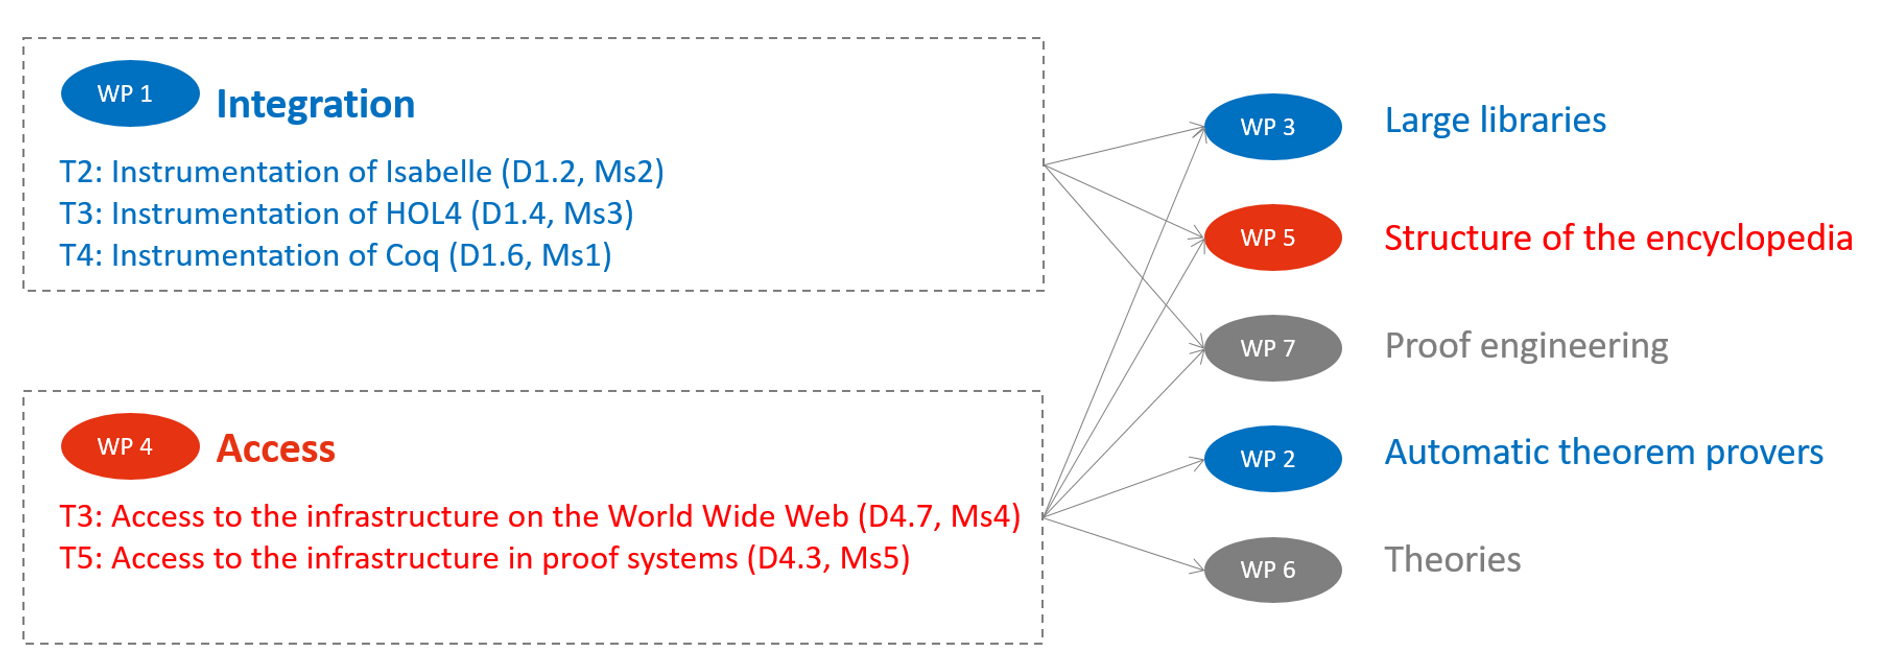
\includegraphics[width=\textwidth]{img/PERT-reduced}


%%% Local Variables:
%%%   mode: latex
%%%   mode: flyspell
%%%   ispell-local-dictionary: "english"
%%% End:
